\documentclass[a4paper,12pt,titlepage]{article}

\usepackage[german,ngerman]{babel}
\usepackage{fontspec}
\setmainfont{Calibri}
\usepackage{graphicx}
\usepackage{hyperref}
\usepackage{caption}

\begin{document}

\begin{titlepage}
    \centering
    \vspace*{2cm}
    {\LARGE\bfseries Automaten und formale Sprachen Blatt 1\par}
    \vspace{2cm}
    {\Large Jan Luca Agricola (275867) \& Jakob Schulz (275258)\par}
    \vspace{2cm}
    {\large\today\par}
\end{titlepage}

\section{Aufgabe}
\begin{enumerate}
\item $\{a, 0\}^*_1 = \{a, 0\}$
\item $\{a, 0\}^*_2 = \{a0, 0a, aa, 00\}$
\item $\{a, b, c\}^+_3 = \{aaa, aab, aac, aba, abb, abc, aca, acb, acc, baa, bab, bac,\\
bba, bbb, bbc, bca, bcb, bcc, caa, cab, cac, cba, cbb, cbc, cca, ccb, ccc\}$
\item $\{a\}^* = \{\epsilon, a, aa, aaa, aaaa,...\}$
\item $\{b\}^* = \{\epsilon, b, bb, bbb, bbbb,...\}$
\item  $\{a, b\}^* = \{\epsilon, a, b, aa, bb, ab, ba, aaa, bbb, aab, ...\}$
\end{enumerate}
\section{Aufgabe}
\begin{enumerate}
\item $\{a\}^* \cup \{b\}^*  = \{a, b\}^*$\\
Falsch, denn $\{a, b\}^*$ hat auch $ab$ als Wort. Dieses Wort kann mit  $\{a\}^* \cup \{b\}^*$ nicht erzeugt werden
\item $\{a\}^* \cup \{b\}^*  \subseteq \{a, b\}^*$\\
Richtig, denn jedes Wort von $\{a\}^* \cup \{b\}^*$ kann auch mit $\{a, b\}^*$ erzeugt werden
\item $\{a\}^* \cap \{b\}^* \cap \{c\}^*  = \{\}$\\
Falsch. Richtig wäre:  $\{a\}^* \cap \{b\}^* \cap \{c\}^*  = \{\epsilon\}$
\item $\{a, b\} \cap \{b, c\}^* = \{b\}^*$\\
Falsch, denn die Schnittmenge kann nur ein Wort bestehend aus $\{b\}$ sein. $\{a, b\}$ hat kein $*$
\end{enumerate}
\section{Aufgabe}
\begin{enumerate}
\item Falsch. Gegenbeispiel: $v = \{abbbb\}, w = \{aab\}$
\item Falsch, was wenn $v = \{aaa\}$ und $w = \{bbb\}$, dann wären beide gleich lang, aber nicht die gleichen Wörter
\item Richtig, wenn man die Längen der einzelnen Wörter addiert, dann ist das dieselbe Länge, wie wenn man die Wörter aneinander hängen würde und dann die Länge bestimmen würde
\item Richtig, wenn u ein Teilwort von v und v ein Teilwort von w ist dann ist u auch ein Teilwort von w.
\item Falsch, denn es gilt: $(ab)^4 = abababab$
\item Richtig, wenn v mehr a hätte als w, dann könnte es kein Teilwort mehr sein und die erste Bedingung wäre nicht mehr gegeben.
\item Richtig, wenn beide Wörter Teilwörter voneinander sind, dann müssen sie die gleichen Wörter sein
\item Ja, es gibt ein Wort u, sodass für alle Wörter gilt $u \cdot v = v \cdot u$. Das Wort u ist das Leerewort ($\epsilon$)
\item Diese Behauptung ist richtig, da eine Konkatenation assoziativ ist
\item Diese Behauptung ist falsch, da eine Konkatenation im Allgemeinen nicht kommutativ ist
\end{enumerate}
\section{Aufgabe}
Den Code finden Sie in der hochgeladenen Java Datei.\\
\\
\\
Alle Tests funktionieren:\\
\\
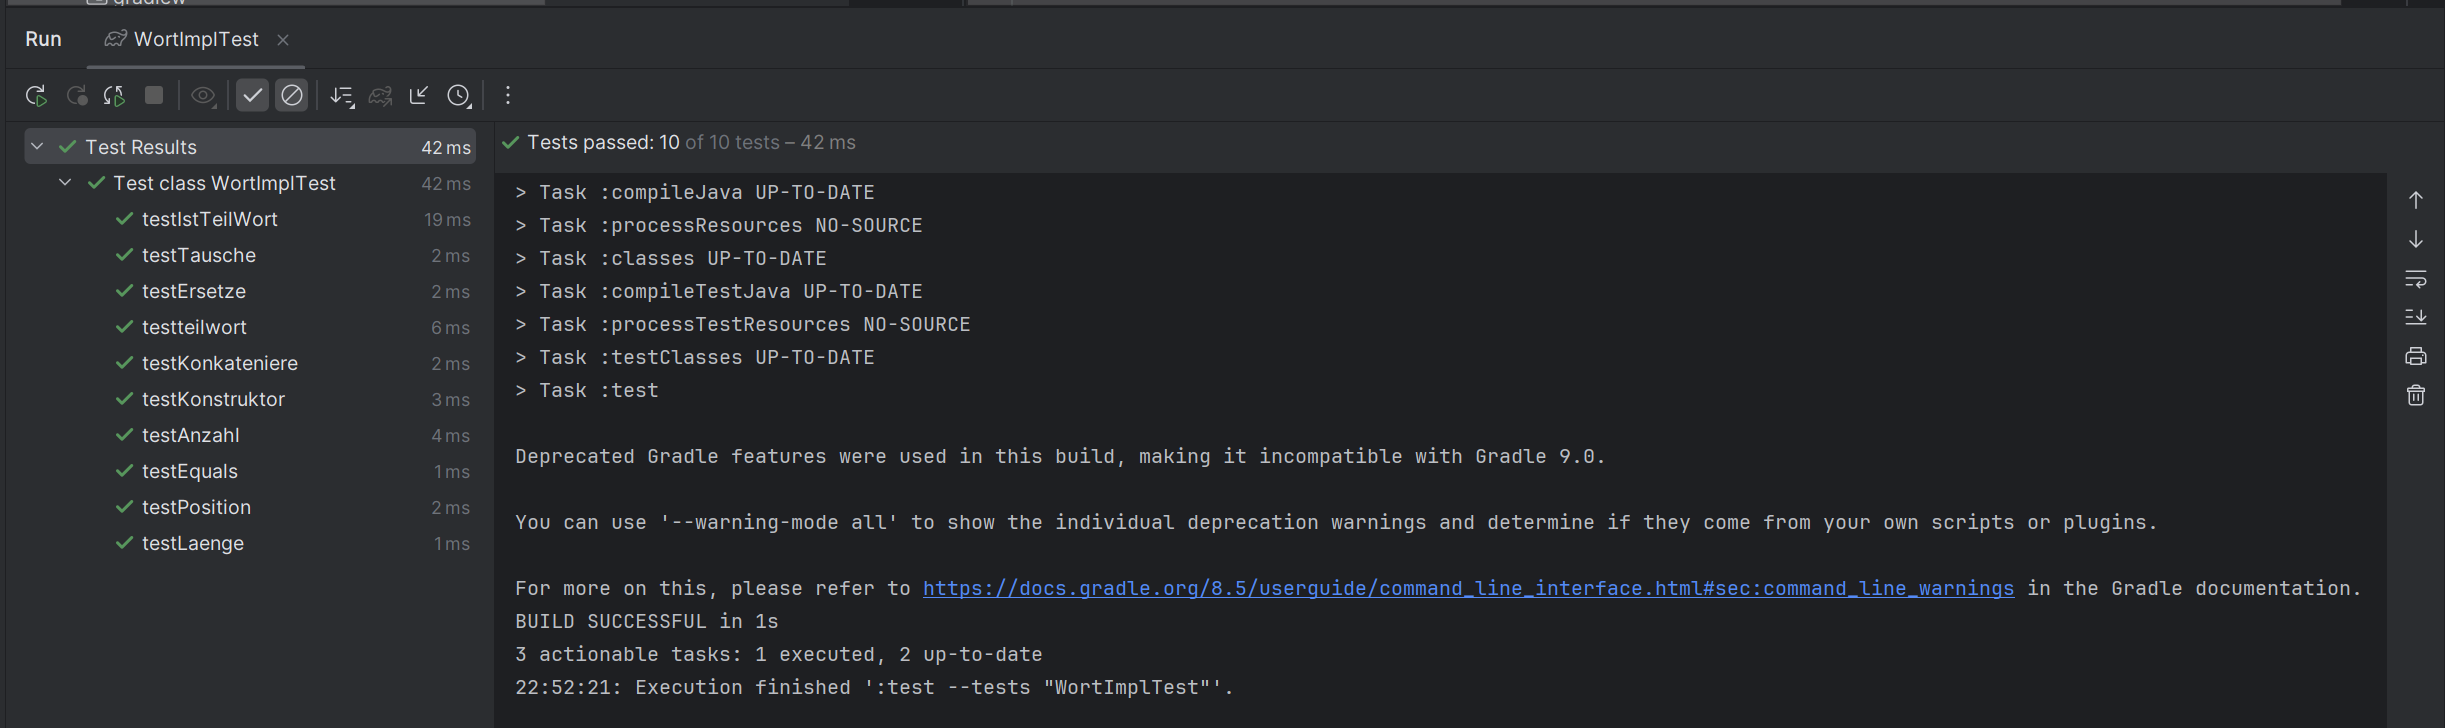
\includegraphics[width=0.9\textwidth]{passedTests.png}
\end{document}
